\documentclass[a4paper, 12pt]{report}
\usepackage[utf8]{inputenc}    
\usepackage[T1]{fontenc}
\usepackage[french]{babel}
\usepackage{hyperref}
\usepackage{setspace}
\usepackage{newtxtext,newtxmath}
\usepackage[top=3cm, bottom=3cm, left=3cm, right=3cm]{geometry}
\usepackage[explicit]{titlesec}
\usepackage{graphicx}
\usepackage[stable]{footmisc}
\usepackage{wrapfig}
\usepackage{multicol}
\usepackage{minitoc}
\usepackage{plantuml}
\usepackage{listings}
\usepackage{array}
\usepackage{pict2e}
\usepackage{slashbox}

\titleformat{\chapter}[display]{}{}{0pt} {
  \parbox{\textwidth} {
    \textbf{\fontsize{30}{30}\selectfont\thechapter.\hspace{0.5cm}\LARGE#1}\\
    \rule{\textwidth}{0.4pt}
  }
}
\titleformat{name=\chapter,numberless}[display]{}{}{0pt} {
  \parbox{\textwidth}{
    \LARGE\textbf{#1}\\
    \rule{\textwidth}{0.4pt}
  }
}

\hypersetup{
    colorlinks=true,
    urlcolor=black,
    linkcolor= black,
    citecolor=black
}

\mtcsetrules{*}{off}

\onehalfspacing

\definecolor{backcolor}{rgb}{0.95,0.95,0.95}
\definecolor{numbers}{rgb}{0.5,0.5,0.5}
\lstdefinestyle{mystyle}{
    backgroundcolor=\color{backcolor},   
    aboveskip=3mm,
    belowskip=3mm,
    showstringspaces=false,
    columns=flexible,
    basicstyle={\small\ttfamily},
    numbers=none,
    breaklines=true,
    breakatwhitespace=true,
    tabsize=3,
    framexleftmargin=16pt,
    framextopmargin=6pt,
    framexbottommargin=6pt, 
    frame=tb, 
    framerule=0pt,
    numbers=left,
    numbersep=20pt,
    numberstyle=\tiny\color{numbers},
}
\lstset{style=mystyle}

\begin{document}
\renewcommand \partname{\thispagestyle{empty}}
\doparttoc

\thispagestyle{empty}
\begin{singlespace}
\begin{center}  
\begin{multicols}{2}
  \flushleft
  \null
  
\includegraphics[width=\columnwidth]{../res/logo-iut.png}
  \flushright
  \null
  \vspace{0.3cm}
  \large{Promotion 2020-2021}
\end{multicols}
\vspace{2cm}
\LARGE{\textit{Mise en place de traitements asynchrones relatifs à la relève des compteurs communiquants}}\\
\vspace{2cm}
\large{\textbf{Mémoire présenté en septembre 2021 par}}\\
\vspace{0.5cm}
\Large{\textit{Loïc STEINMETZ}}\\
\vspace{2cm}
\large{\textbf{En vue de l'obtention de la Licence Professionnelle}}\\
\vspace{0.5cm}
\fbox{
  \begin{minipage}{12cm}
    \begin{center}
      \null
      \vspace{0.3cm}
      \textbf{Métiers de l'Informatique}\\
      Conception, développement et test de logiciels\\
      Parcours Métiers du Génie Logiciel\\
      \null
    \end{center}
  \end{minipage}
}
\vspace{2.8cm}
\begin{multicols}{2}
  \flushleft
  \null
  \textbf{Alternance effectuée à :}\\
  Efluid\\
  2 bis, rue Ardant du Picq\\
  CS 10100 57004 METZ Cedex 01\\
  \flushright
  \null
  
\includegraphics[width=.6\columnwidth]{../res/logo-efluid.jpg}
\end{multicols}
\end{center}
\end{singlespace}

\clearpage
\thispagestyle{empty}
\null
\clearpage

\begin{singlespace}
\thispagestyle{empty}
\begin{center}  
\begin{multicols}{2}
  \flushleft
  \null
  
\includegraphics[width=\columnwidth]{../res/logo-iut.png}
  \flushright
  \null
  \vspace{0.3cm}
  \large{Promotion 2020-2021}
\end{multicols}
\vspace{2cm}
\LARGE{\textit{Mise en place de traitements asynchrones relatifs à la relève des compteurs communiquants}}\\
\vspace{2cm}
\large{\textbf{Mémoire présenté en septembre 2021 par}}\\
\vspace{0.5cm}
\Large{\textit{Loïc STEINMETZ}}\\
\vspace{2cm}
\large{\textbf{En vue de l'obtention de la Licence Professionnelle}}\\
\vspace{0.5cm}
\fbox{
  \begin{minipage}{12cm}
    \begin{center}
      \null
      \vspace{0.3cm}
      \textbf{Métiers de l'Informatique}\\
      Conception, développement et test de logiciels\\
      Parcours Métiers du Génie Logiciel\\
      \null
    \end{center}
  \end{minipage}
}
\vspace{2.8cm}
\begin{multicols}{2}
  \flushleft
  \null
  \textbf{Alternance effectuée à :}\\
  Efluid\\
  2 bis, rue Ardant du Picq\\
  CS 10100 57004 METZ Cedex 01\\
  \flushright
  \null
  
\includegraphics[width=.6\columnwidth]{../res/logo-efluid.jpg}
\end{multicols}
\end{center}
\end{singlespace}

\chapter*{Remerciements}
\addcontentsline{toc}{chapter}{Remerciements}
\thispagestyle{empty}

Je remercie tout particulièrement mon maître de stage, Alexandre L'Huillier, pour m'avoir fait bénéficier de ses compétences tout au long de mon année d'alternance. Merci à lui pour son professionalisme, sa confiance et sa disponibilité.

Je remercie également Jean-Luc Thiry, chef de service et Didier Grzejszczak, chef de filière, pour leur accompagnement général et pour ma bonne intégration au sein de l'entreprise.

Mes remerciements vont enfin à l'ensemble des membres du service auquel j'ai été intégré et que je n'ai pas encore cités : Patrice Frantz, Julien Kempf, Fabienne Mamet, François Molin, Roderick Pierre, Stéphane Poirot et Stéphane Roedel.

\part{Mémoire}
\renewcommand{\clearpage}{}
\chapter*{Sommaire}
\renewcommand\ptctitle{}
\parttoc
\thispagestyle{empty}
\renewcommand{\clearpage}{\newpage}
\clearpage

\chapter*{Abstract}
\addcontentsline{toc}{chapter}{Abstract}

During this year of apprenticeship, I was integrated in \textit{Efluid} company, an UEM's subsidiary based in Metz which provides a software package solution covering all requirements of electricity, gas and water stakeholders. The department I was integrated in is in charge of the consumption management domain.\\

\textit{Efluid} allows one main programming language, \textit{Java}. Besides this language, SQL is required too, in order to handle database operations. When I joined the company, I had already worked with these languages which facilitated my primary integration in the general \textit{Efluid}'s workflow.\\

I was personaly responsible for the conception and implementation of a batch process which was intended to improve the software performance. The project consisted in moving some of the existing process from a real time execution context to an asynchronous and periodicaly launched program. The involved process was actualy the consumption reading's publication management, whose purpose is to prepare the communication with partners like global network managers or regulatory entities.

Besides this main project, I contributed to the current development tasks which are distributed every week among the team members. I had then to fix some minor bugs and to implement a few new features. These tasks allowed me to have a better understanding of my developement environnment and the software's structure.\\

This professional experience made me learn how a complex application like \textit{Efluid} can be managed. I especialy discovered how the methods can evolve, from an individual school project to a fully integrated production workflow involving a real distribution and a proper maintenance.

\chapter*{Introduction}
\addcontentsline{toc}{chapter}{Introduction}

Ce mémoire a pour objectif de présenter les travaux réalisés dans mon entreprise d'accueil, \textit{Efluid}, dans le cadre de la licence professionnelle génie logiciel, réalisée en alternance. Cette année fait suite à l'obtention de mon DUT informatique réalisé en année spéciale.

Ayant déjà réalisé mon stage de fin de DUT chez \textit{Efluid}, j'ai pu rapidement postuler à l'une des offres d'alternance que proposait le service qui m'avait déjà accueilli. Dans la continuité de mes treize semaines de stage, j'ai alors pu réintégrer ce même service pour mon année d'alternance.\\

C'est donc au sein de la division "consommation" et sous la tutelle d'Alexandre L'Huillier que j'ai pu travailler sur le projet qui m'a été confié. Je reviendrai plus loin sur la place du service dans l'organisation d'\textit{Efluid} et sur le détail du projet. On peut néanmoins résumer ainsi la formulation initiale du projet : Il s'agissait de déporter une partie des traitements réalisés en temps réel par le logiciel dans des processus asynchrones.

Afin de mieux comprendre les enjeux et les objectifs de ce projet, je commencerai par présenter l'entreprise et son activité. Je détaillerai ensuite la nature des différentes tâches qui m'ont été confiées, ce qui me permettra de décrire le cadre de mes travaux : mon environnement de développement et les différents processus de production de l'entreprise. 

Il s'agira donc ensuite de détailler la mise en oeuvre du projet principal qui m'a été confié. J'expliquerai alors les différents aspects techniques et fonctionnels de mes travaux dans l'ordre de leur réalisation. Je présenterai ainsi la méthode générale mise en oeuvre et dont découle précisément cet enchaînement. 

Je concluerai enfin en présentant les différents apports de cette année d'alternance dans la perspective plus générale de mon parcours professionnel.

\chapter{Présentation de l'entreprise}

\begin{figure}[t]
  \begin{center}
    \begin{minipage}{4cm}
      \begin{center}
        
\includegraphics[height=2cm]{../res/logo-efluid.jpg}
        \caption{Efluid}
        \label{efluid}
      \end{center}
    \end{minipage}
    \rule{1cm}{0cm}
    \begin{minipage}{4cm}
      \begin{center}
        
\includegraphics[height=2cm]{../res/logo-uem.jpg}
        \caption{UEM}
        \label{uem}
      \end{center}
    \end{minipage}
    \rule{1cm}{0cm}
    \begin{minipage}{4cm}
      \begin{center}
        
\includegraphics[height=2cm]{../res/logo-enedis.jpg}
        \caption{Enedis}
        \label{enedis}
      \end{center}
    \end{minipage}
  \end{center}
\end{figure}

\section{Présentation générale}

\textit{Efluid} (\textit{cf.} figure \ref{efluid}) est une société éditrice de logiciel. Le produit qu'elle développe, portant le même nom, est un progiciel à destination des entreprises du secteur de l'énergie, qu'il s'agisse des gestionnaires de réseaux ou des distributeurs d'électricité (\textit{cf.} Annexe \ref{appendix:logiciel} : Le logiciel \textit{Efluid}). Il s'agit d'un ERP\footnote{\textit{Enterprise Resource Planning}}, ou logiciel de gestion intégré, pensé pour être adapté aux besoins spécifiques de ce secteur. Le programme est donc conçu pour pouvoir intégrer tous les aspects de cette activité, de la gestion des contrats d'énergie à la comptabilité, de la gestion des stocks de matériels à l'édition de documents légaux. La structure du programme est modulaire et permet donc aux clients de l'entreprise d'adapter la solution à leur besoin.\\

Cette dimension modulaire de l'application donne lieu à une division fonctionnelle des services de développement de la société, c'est-à-dire à un regrouppement des activités de développement non pas selon un critère technique (suivant par exemple l'opposition \textit{front-end}/\textit{back-end}), mais d'après les solutions apportées dans les domaines concrets de l'activité des clients (\textit{cf.} Annexe \ref{appendix:efluid-organisation} : L'organisation des services d'\textit{Efluid}). J'ai donc pour ma part été intégré à la division "consommation", qui appartient elle-même au service "comptage et réseaux". 

Outre les services de développements fonctionnels dans lesquels sont intégrés la majorité des développeurs, il existe également des services chargés de missions transverses, comme par exemple le déploiement de l'application ou le développement des composants élémentaires du programme. C'est une partie du processus de production que j'ai moins été en mesure d'aborder au cours de mon année d'alternance, mais avec laquelle j'ai néanmoins été en contact, puisque certains de ces services sont aussi chargés de la gestion des environnements de développement et de la maintenance des infrastructures de \textit{versionning}.\\

\textit{Efluid} a été développé à l'initiative de l'UEM (\textit{cf.} figure \ref{uem}), en partenariat avec \textit{Enedis} (\textit{cf.} figure \ref{enedis}), qui émane d'EDF (\textit{cf.} Annexe \ref{appendix:efluid-gouvernance} : La gouvernance d'\textit{Efluid}) et profite donc de l'expertise de ces groupes afin de répondre au mieux aux besoins du secteur de l'énergie. La société est devenu un acteur important dans la gestion des systèmes d'information de ce secteur et emploie aujourd'hui plus de deux-cent agents. \textit{Efluid} compte \textit{Enedis} parmi ses clients mais aussi un grand nombre de régies locales dont par exemple l'\textit{Electricité de Strasbourg}. L'entreprise répond également a des appels d'offre à l'étranger et pourrait donc à terme prendre une dimension internationale.

\section{Spécificités du logiciel}

D'un point de vue technique, la solution applicative d'\textit{Efluid} (ou "suite \textit{Efluid}") est composée de différents modules, intégrés différement en fonction du besoin client :\\

\textit{La liste suivante est non exhaustive.}

\begin{itemize}
  \item \textit{efluid} : traitements métiers et interface web
  \item \textit{suivefluid} : application de gestion d'événements
  \item \textit{efluid.net} : gestion des échanges avec les systèmes d'information
  \item \textit{mobefluid} : application mobile
\end{itemize}
\vspace{0.5cm}

Dans le cadre des travaux qui m'ont été affectés, j'ai été amené à travailler sur des modules techniques qui subdivisent le module \textit{efluid} proprement dit : \textit{Ecore}, \textit{Efluid}, \textit{Interfaces} et \textit{Batch}. Conformément à mon affectation j'ai abordé principalement le domaine "consommation" au sein de ces différents modules. Il convient donc d'en mentionner les spécificités fonctionnelles.

Le traitements des consommations est une partie importance du logiciel, et consiste notamment à assurer la bonne gestion des relèves. Les relèves peuvent être de différents types, selon la nature des acteurs et des activités impliquées. En effet, une relève peut correspondre à une activité de consommation ou de production, à une mesure électrique ou gazière, être réalisée via l'intervention d'un agent, un relevé effectué par le client lui-même, ou via un compteur communiquant. Il ne s'agit là que de quelques critères parmi tous ceux qui peuvent impacter les traitements à réaliser. La gestion des relèves est donc gérée via un système complexe qui implique également de nombreux processus de calcul permettant d'intégrer les différentes grandeurs mesurées en respectant les contraintes liées à leur nature physique ainsi que les contraintes réglementaires. Conformément à la réglémentation en vigueur, toutes ces mesures doivent également pouvoir être communiquées aux différents acteurs impliqués : fournisseurs, gestionnaires de concession, clients finaux, organismes de contrôle, etc.

Ne disposant que d'une connaissance très partielle de ces différentes contraintes fonctionnelles, je ne peux pas toutes les lister ici ; une présentation détaillée de ces contraintes dépasserait en outre le cadre de ce mémoire. Cette brève description des spécificités métiers régissant le domaine consommation me permet néanmoins d'insister sur la grande complexité des traitements mis en oeuvre. On peut également noter que c'est dans la réponse à l'ensemble de ces contraintes, qu'il s'agisse de celle du domaine "consommation" ou non, que l'expertise de l'UEM a été déterminante.

Outre la grande compléxité des cas d'utilisation auxquels répond \textit{Efluid}, la solution proposée doit également répondre de certaines normes techniques négociées avec les différents clients et qui donnent lieu à des impératifs contractuels. Parmi ces spécifications techniques, on peut notamment citer les contraintes de performance auxquelles doit répondre le logiciel. Certains temps de traitement doivent par exemple correspondre à des seuils pré-déterminés, et la non-conformité des mesures de performance peut se traduire par des pénalités financières.\\

D'un point de vue général, \textit{Efluid} consiste donc en une solution applicative particulièrement complexe, ayant à répondre de nombreuses contraintes, qu'elles soient techniques ou fonctionnelles. Ce sont ces contraintes qui imposent la réalisation d'une maintenance en continu des différents traitements et l'intégration régulière de nouveaux processus. C'est précisément dans le cadre de ces contraintes générales et des contraintes propres au domaine "consommation" que s'inscrit le projet que j'ai eut à gérer. Je présenterai donc plus en profondeur certains aspects fonctionnels au moment de détailler ses objectifs.

\chapter{Sujets traités}

\section{Généralités}

Dans le cadre de mes travaux, j'ai pu appréhender l'environnement de développement propre à \textit{Efluid}, qu'il s'agisse des outils et logiciels utilisés, ou des processus de production mis en place.

\begin{figure}[b]
  \begin{center}
    \begin{minipage}{4cm}
      \begin{center}
        
\includegraphics[height=2cm]{../res/java.jpg}
        \caption{Java}
        \label{java}
      \end{center}
    \end{minipage}
    \rule{1cm}{0cm}
    \begin{minipage}{4cm}
      \begin{center}
        
\includegraphics[height=2cm]{../res/oracle.png}
        \caption{Oracle}
        \label{oracle}
      \end{center}
    \end{minipage}
    \rule{1cm}{0cm}
    \begin{minipage}{4cm}
      \begin{center}
        
\includegraphics[height=2cm]{../res/intellij.jpg}
        \vspace{0.1cm}
        \caption{Intellij}
        \label{intellij}
      \end{center}
    \end{minipage}
  \end{center}
\end{figure}

\subsection{Environnement de développement}

L'application \textit{Efluid} est développée en \textit{Java} (\textit{cf.} figure \ref{java}). C'est un langage dont j'avais déjà une certaine maîtrise avant de rejoindre l'entreprise et je n'ai donc pas eut à suivre de formation dédiée. Au delà du langage utilisé, \textit{Efluid} est  basé sur une architecture et un \textit{framework} complexe, développé initialement par CGI. La familiarisation avec la structure générale de l'application a quant à elle été plus longue et a nécessité un suivi continu durant mon année d'alternance. 

J'ai en outre bénéficié d'une formation fonctionnelle sur le logiciel, destinée aux nouveaux entrants et aux clients d'\textit{Efluid}, portant donc sur l'utilisation proprement dite du logiciel. Je n'ai pour ma part suivi que la formation qui portait sur le fonctionnement du domaine "consommation" ; celle-ci m'a permis de mieux appréhender les différentes fonctionnalités du logiciel ainsi que le fonctionnement général de l'application.

Outre le \textit{Java}, j'ai aussi été amené à mobiliser mes compétence en \textit{SQL}. La base de données d'\textit{Efluid} est en effet une base \textit{Oracle} (\textit{cf.} figure \ref{oracle}) et implique donc la programmation de requêtes SQL et d'autres processus en PL/SQL, le langage propre aux bases de données \textit{Oracle}.

Les principaux logiciels que j'ai été amené à utiliser ont ainsi été \textit{Intellij} (\textit{cf.} figure \ref{intellij}) et \textit{SQL Developper}. Ce sont deux logiciels avec lesquels j'étais déjà familier et sur lesquels j'ai néanmoins été amené à approfondir mes compétences. J'ai enfin été amené à utiliser \textit{Git} comme outil de \textit{versionning}. L'intégration de \textit{Git} dans les processus de production d'\textit{Efluid} m'a permis d'appréhender une utilisation plus avancée de cet outil.

\begin{figure}[b]
  \begin{center}
    \begin{minipage}{4cm}
      \begin{center}
        \vspace{0.5cm}
        
\includegraphics[height=1cm]{../res/git.png}
        \null
        \vspace{0.5cm}
        \caption{Git}
        \label{git}
      \end{center}
    \end{minipage}
    \rule{1cm}{0cm}
    \begin{minipage}{4cm}
      \begin{center}
        
\includegraphics[height=2cm]{../res/jenkins.png}
        \caption{Jenkins}
        \label{jenkins}
      \end{center}
    \end{minipage}
    \rule{1cm}{0cm}
    \begin{minipage}{4cm}
      \begin{center}
        \vspace{0.5cm}
        
\includegraphics[height=1cm]{../res/maven.png}
        \null
        \caption{Maven}
        \label{maven}
      \end{center}
    \end{minipage}
  \end{center}
\end{figure}

\subsection{Processus de production}

Les processus de production mis en place par \textit{Efluid} reposent principalement sur quatre outils :\\

\begin{itemize}
  \item \textit{Suivefluid}
  \item \textit{Git} (\textit{cf.} figure \ref{git}), utilisé avec \textit{Gerrit}
  \item \textit{Maven} (\textit{cf.} figure \ref{maven})
  \item \textit{Jenkins} (\textit{cf.} figure \ref{jenkins})
\end{itemize}
\vspace{0.5cm}

\textit{Suivefluid} est un logiciel de suivi d'événements développé en interne et qui assure la coordination des différents services : relation client, recette et développement. Chaque développement correspond ainsi à un un événement qui se retrouve affecté à un service de développement puis à un développeur.

Suite à la réalisation du développement en question, les modifications du code sont alors synchronisées via \textit{Git}, et donnent lieu à une revue de code via \textit{Gerrit}. Une fois le développement validé, celui-ci peut alors être intégré au code source de l'application. A noter que différentes branches de développement sont gérées en même temps compte-tenu des versions en production chez les différents clients. Outre la branche de développement principale, des branches de maintenance sont en effet destinées à assurer le suivi d'anciennes versions de l'application lorsque celle-ci sont encore utilisées par certains clients.

L'ensemble des processus d'intégration et de déploiement continus sont par ailleurs administrés via \textit{Jenkins}, cet outil permettant notamment d'automatiser la compilation, les tests et le packaging de l'application. En dernière instance, ces processus sont basés sur des scripts \textit{Maven}. En effet, \textit{Maven} permet d'encapsuler l'ensemble de la configuration propre à l'application, via des fichiers POM\footnote{\textit{Project Object Model}}, qui décrivent les différentes phases du cycle de production.\\

L'utilisation de ces outils et l'intégration plus générale des processus de production d'\textit{Efluid} m'ont permis d'appréhender les méthodes de gestion d'un projet complexe, qu'il s'agisse de son administration générale ou de la mise en place de processus de test ou de contrôle qualité. C'est donc dans ce cadre que j'ai du réaliser mes différents travaux.

\section{Développements courants}

En parallèle de mon projet principal, sur lequel je reviendrai, j'ai été amené à traiter certains événements courants. Les événements donnant lieu à un développement sont répartis chaque semaine entre les différents développeurs du service et les travaux peuvent concerner de nombreux aspects de l'application : \\

\begin{itemize}
  \item IHM \footnote{Interface Homme Machine}
  \item Traitements et algorithmes
  \item Gestion des données
  \item Gestion des logs
  \item Gestion du \textit{routing} et de la navigation
  \item \textit{Refactoring} du code existant
  \item Ecriture ou adaptation de tests
  \item Etc...
\end{itemize}
\vspace{0.5cm}

Certains projets plus longs nécessitent de passer par des procédures plus complexes, impliquant notamment les services d'analyse. La mise en oeuvre de tels projet peut alors impliquer un découpage technique : plusieurs événements peuvent correspondre à un même projet et être répartis entre plusieurs développeurs.\\

J'ai pour ma part eut à traiter notamment des corrections d'anomalies, des nouveaux développements mineurs et des travaux de \textit{refactoring}. J'ai en effet du corriger certaines anomalies au niveau de l'interface de l'application, ce qui m'a permis de mieux appréhender l'architecture générale de l'application. J'ai également du intégrer de nouveaux attributs à certains objets métiers, ce qui m'a cette fois permis d'approfondir la logique de gestion de la persistance des données. J'ai enfin eut à gérer des événements de \textit{refactoring} qui m'ont permis quant à eux de mieux comprendre certains processus et traitements du logiciel, et d'approfondir ma compréhension des tests unitaires et des tests d'intégration.

D'une manière générale, la gestion de ces événements m'a permis de me familiariser progressivement avec le \textit{framework} d'\textit{Efluid}. A travers ces différents travaux, j'ai en effet été amené à approfondir les différentes couches de l'architecture du logiciel, ce qui s'est avéré être très utile au moment d'aborder mon projet. C'est également à travers la gestion de ces événements que j'ai pu me familiariser avec l'ensemble des processus mis en place ainsi qu'avec les conventions et la démarche qualité propres à \textit{Efluid}. La revue de code systématique à laquelle donnent lieu les développements m'a en outre fait gagner en compétence d'un point de vue technique. J'ai en effet pu bénéficier de l'expertise des différents relecteurs concernant la logique générale de mes développements, l'utilisation de certains patrons de conception et le respect des bonnes pratiques de développement.

\section{Projet principal}

Comme indiqué en introduction, le projet principal qui m'a été attribué consistait à déporter une partie des traitements réalisés en temps réel par le logiciel dans un \textit{process} asynchrone. En d'autres termes, mon projet consistait à pouvoir gérer ces traitements en mode \textit{batch}, au lieu de les intégrer aux processus réalisés "au fil de l'eau". Dans la suite de ma présentation j'utiliserai de manière indistincte la terminologie suivante :\\

\begin{itemize}
  \item "Traitement \textit{batch}", "traitement asynchrone" : Processus automatisé, portant sur un ensemble souvent massif de données marquées spécifiquement pour donner lieu à certains traitements.
  \item "Traitement au fil de l'eau", "traitement synchrone" : Traitement réalisé en temps réel suite à une action utilisateur, dont le résultat est visible immédiatement et portant uniquement sur les informations d'un contexte applicatif spécifique.
\end{itemize}
\vspace{0.5cm}

De nombreux \textit{batchs} sont intégrés à la solution applicative d'\textit{Efluid}. Comme indiqué dans la présentation générale du logiciel, les mesures de performance de l'application donnent lieu à des impératifs contractuels. Le recours à des traitements \textit{batchs} permet donc d'alléger les opérations réalisées de manière synchrone et donc d'écourter les temps de chargement lors du parcours utilisateur. Le gain de performances constituait ainsi le principal objectif de mon projet, et ce concernant un traitement en particulier correspondant à la demande de publication de la relève.

D'un point de vue fonctionnel, la demande de publication consiste à déterminer, à partir d'une relève, si les mesures enregistrées doivent être communiquées à des acteurs externes selon des critères prédéfinis et, le cas échéant, à associer à la relève un objet portant les informations de publication. A noter que la publication proprement dite, à savoir la transmission effective des données aux acteurs concernés, est réalisée par un \textit{batch} dédié ; le périmètre de la demande de publication s'arrête quant à lui au marquage des relèves qui nécessitent une publication. Dans la situation initiale, la demande de publication était donc gérée intégralement au fil de l'eau, ce qui entrainait des temps de traitements trop longs, pouvant excéder les objectifs de performance. L'implémentation d'un \textit{batch} dédié à la demande de publication avait donc pour objectif d'alléger ces temps de traitement.\\

L'autre objectif de mon projet consistait à réorganiser les appels de la demande de publication de la relève. Initialement, la demande de publication était en effet appelée au cours de différents processus dispersés dans le code de l'application. Les traitements étaient donc répétés et pouvaient donner lieu à des implémentations différentes selon les contextes. Outre le gain de performance, mon projet avait donc également pour but d'implémenter un point d'accès unique à la demande de publication.

J'expliquerai plus loin pourquoi cet objectif a finalement été partiellement abandonné. Il a en effet était jugé préférable de se concentrer d'abord sur le gain de performance potentiel pouvant être réalisé.\\

Le projet tel qu'il m'a été confié était encore en cours d'étude. En amont des travaux d'implémentation, il a donc donné lieu à une longue phase d'analyse. Une fois cette analyse réalisée, la conception technique de la solution et l'implémentation des nouveaux traitements ont été réalisés en parallèle (\textit{cf.} annexe \ref{appendix:planification} : Planification générale). Je présenterai donc le traitement de mon projet industriel de manière chronologique.

\chapter{Traitement du projet industriel}

\section{Analyses préliminaires}

La première phase du projet consistait à évaluer les différentes contraintes liées à l'implémentation du \textit{batch} de demande de publication de la relève. Les analyses préliminaires ont notamment permis de dégager la volumétrie des traitements associés à la demande de publication et de décrire les différents contextes d'appels de ces traitements. Elle a par ailleurs conduit à la formalisation d'un planning de travail plus détaillé.

\subsection{Analyse volumétrique}

L'analyse de la volumétrie de la demande de publication avait pour objectif de dégager l'intérêt de la solution proposée en termes de performances, et d'évaluer sa faisabilité.\\

Cette analyse a nécessité la formalisation de requêtes SQL permettant d'évaluer le nombre de relèves donnant lieu à une demande de publication. Il a ainsi été possible de déterminer l'impact des modifications potentielles en ce qui concerne la quantité de données à traiter : \textit{cf.} annexe \ref{appendix:volumetrie}, analyse volumétrique. Il faut notamment retenir de cette évaluation la grande quantité de données en jeu : les systèmes d'information des différents clients peuvent en effet avoir à gérer plusieurs millions de relèves et de demandes de publication par mois.

L'importance de la quantité de données à traiter a également eut un impact sur l'implémentation et le plan d'intégration du \textit{batch} qu'il s'agissait de mettre en place. Tout comme les opérations gérées au fil de l'eau, les traitements \textit{batch} doivent respecter certains objectifs de performances. L'ensemble des \textit{batchs} doit en effet respecter un temps maximal d'exécution.

\subsection{Analyse des contextes de demande de publication de la relève}

En parallèle de l'analyse volumétrique, il a également été nécessaire de lister et de reproduire les différents contextes applicatifs dans lesquels était appelée la demande de publication : \textit{cf.} annexe \ref{appendix:process}, contextes de la demande de publication.\\

L'identification de ces différents contextes a ainsi permis de mieux cerner les implications potentielles d'une modification des traitements existants. La reproduction des contextes a par ailleurs servi à tester la non-régression de l'implémentation et à identifier les données nécessaires pour l'exécution de chaque traitement. 

Dans le cadre d'un traitement en mode \textit{batch}, il faut en effet noter que l'ensemble des données nécessaire aux processus appelés doit être chargé avant leur exécution. Il était donc important de pouvoir cerner les aspects fonctionnels propres à chaque contexte, de sorte que les traitements asynchrones puissent répliquer les traitements prévus. L'un des principaux critère à prendre en compte a par exemple été la distinction entre les relèves validées via un compte-rendu d'intervention (CRI) ou via d'autres processus. Mais il ne s'agit là que d'un des critères ayant une influence sur la demande de publication.

L'analyse détaillée du processus de demande de publication a également permis de fournir une description de la structure des traitements. La demande de publication est en effet constituée de \textit{process} complexes et se décompose elle-même en différents sous-traitements déterminés en fonction du contexte et reposant sur un système d'héritage. Cette première phase d'analyse a donc permis d'évaluer les contraintes techniques pesant sur l'intégration du \textit{batch}.

\subsection{Formation \textit{batch}}

Au cours de cette première phase de travail, j'ai également bénéficié d'une formation concernant l'implémentation d'un \textit{batch} dans le cadre du \textit{framework} général d'\textit{Efluid}. Il faut en effet noter que le module \textit{Batch} constitue en lui-même un \textit{framework} impliquant des conventions strictes et une architecture spécifique. Il était donc important d'avoir une compréhension générale du système avant de pouvoir concevoir une solution technique pertinente.

La nature asynchrone des traitements \textit{batch} implique elle aussi certaines contraintes. Outre le chargement préalable de l'ensemble des données nécessaires au bon déroulement des traitements, contrainte que j'ai déjà mentionné, la parallélisation des tâches à laquelle donne lieu ce type de traitement implique une attention toute particulière à la gestion de l'état des données. L'exécution d'un \textit{batch} a en effet lieu sur la base d'un contexte figé, chargé lors de son initialisation. Ce contexte est alors techniquement décorellé du contexte applicatif généré par les opérations des utilisateurs du logiciel. On peut par exemple imaginer dans le cadre du projet en question qu'une relève soit validée et donc chargée par le \textit{batch}, puis qu'elle soit invalidée par un agent pendant l'exécution des traitements asynchrones : Le \textit{batch} n'a alors pas connaissance de la modification du statut de la relève.\\

La formation spécifique au module \textit{batch} dont j'ai pu profiter m'a finalement permis de comprendre l'ensemble des contraintes propres à ce type de traitements. J'ai ainsi pu mieux appréhender leur l'architecture générale, leurs caractéristiques techniques, et certaines de leurs spécificités fonctionnelles.

\section{Formalisation du besoin et planification}

On peut finalement résumer le besoin initial auquel répond le projet par ces deux objectifs :

\begin{itemize}
  \item Réduire les temps de traitement lors de l'utilisation de l'application web
  \item Implémenter un point d'accès unique à la demande de publication de la relève pour l'ensemble des processus de l'application
\end{itemize}

\subsection{Formalisation du périmètre fonctionnel du projet}

Conformément aux processus de production mis en place par l'entreprise, ce projet a d'abord donné lieu à une présentation et une discussion avec les services d'analyse. Deux contraintes principales ont alors été mises en évidence :\\

\begin{itemize}
  \item Contrainte de performance : le \textit{batch} devra être exécuté plusieurs fois par jour et ses temps de traitements doivent permettre de gérer ensuite la publication proprement dite.
  \item Contrainte client : \textit{Enedis}, le principal client d'\textit{Efluid}, souhaite conserver le plus de traitements synchrones possible, ce qui va à l'encontre du projet.
\end{itemize}
\vspace{0.5cm}

Avec l'accord des services d'analyse, et compte tenu de ces contraintes, il a finalement été décidé de réduire le périmètre d'application du projet. En effet, afin de répondre à la contrainte d'acceptabilité du projet posée notamment par \textit{Enedis}, l'objectif de migrer l'ensemble des appels de la demande de publication a finalement été réduit. Le projet a ainsi consisté à ne migrer que la demande de publication réalisée au moment de l'import des relèves des compteurs communiquants d'\textit{Enedis}, ou compteurs \textit{Linky} (\textit{cf.} figure \ref{linky}). Cet import est réalisé via l'interface "LKY06" ; la mention ultérieure de ce \textit{process} renverra donc à l'ensemble du process d'import des relèves \textit{Linky}.

Malgré la réduction du périmètre fonctionnel, il a néanmoins été convenu que cette solution, si elle finissait par être retenu par le client, devait garantir une migration facile des autres processus de demande de publication. Bien que les objectifs initiaux du projet aient été réduits, il a donc fallu tenir compte de la potentielle migration d'autres traitements vers la solution à développer en proposant une implémentation qui puisse être facilement modulable.

\subsection{Description fonctionnelle du \textit{batch}}

\begin{figure}[t]
  \begin{center}
    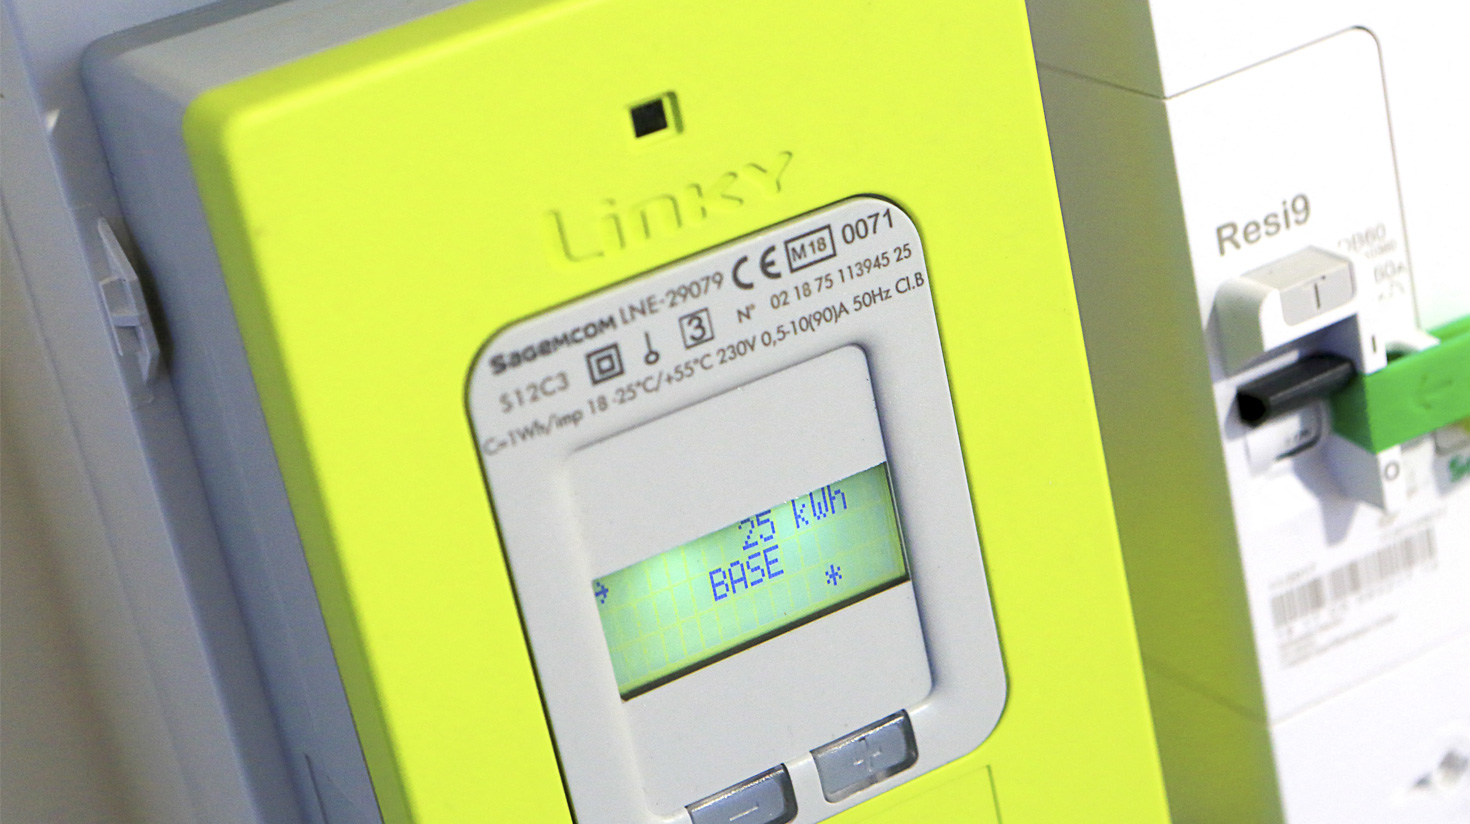
\includegraphics[height=4cm]{../res/linky.jpg}
    \caption{Compteur \textit{Linky}}
    \label{linky}
  \end{center}
\end{figure}

La demande de publication de la relève était initialement gérée au fil de l'eau via différents processus, dont la validation et l'invalidation de la relève. Le \textit{batch}, exécuté régulièrement en journée, devait permettre quant à lui de gérer la demande de publication de façon différée. 

Les traitements réalisés par le \textit{batch} devaient être basés sur les processus de demande de publication existants. Dans le cas d'une demande de publication gérée par \textit{batch}, les modalités devaient donc être identiques à celles d'une demande de publication synchrone telle qu'elle était gérée avant la nouvelle implémentation. Dans ce cas, le processus appelant devait donc se contenter de marquer les relèves concernées afin que le \textit{batch} puisse ensuite les ramasser est réaliser les traitements prévus.

Le traitement différé de la demande de publication implique en outre la gestion de problèmes de concurrence. Les échanges associés à la relève doivent en effet garder un état cohérent par rapport aux opérations réalisées via l'interface du logiciel et ce malgré la gestion asynchrone de la demande de publication.\\

La mise en place de la sélection des relèves, permettant de déporter une partie des demandes de publication vers le \textit{batch}, devait donc prendre en compte deux contraintes majeures :

\clearpage

\begin{itemize}
  \item \textbf{Contraintes de modularité : }
  \begin{itemize}
    \item Les développements visaient à pouvoir sélectionner les relèves enregistrées par l'interface LKY06, dont la demande de publication devaient être gérée de façon asynchrone, mais sans altérer les processus exécutés de manière synchrone dans les autres contextes.
    \item L'intégration devait cependant permettre la migration ultérieure d'autres processus de la demande de publication synchrone vers la demande de publication asynchrone. 
  \end{itemize}
  \vspace{0.5cm}
  \item \textbf{Contrainte d'intégrité :} Afin de garantir la cohérence des opérations réalisées sur les relèves concernées par la sélection, le marquage devait être réalisé lors de la validation des relèves mais aussi lors de leur invalidation. En effet, dans le cas de la validation d'une relève avec gestion asynchrone de la demande de publication, il fallait pouvoir gérer sa potentielle invalidation alors même que la demande de publication n'a pas encore été réalisée. Il fallait également pouvoir gérer les problèmes de concurrence qu'impliquent les traitments asynchrones : si la demande de publication d'une relève est en cours de traitement, il devait être possible d'opérer un retour sur l'opération si dans le même temps la relève était invalidée.
\end{itemize}

\subsection{Découpage technique}

Avant d'aborder les travaux de conception et d'implémentation, j'ai pu procéder à un découpage technique du projet. En prenant exemple sur des implémentations de \textit{batchs} antérieures, j'ai donc pu diviser l'ensemble des travaux en différentes étapes, impliquant pour chacune d'entre elles une phase de conception et une phase de développement. Les différents travaux de conception ont ainsi du être formalisés dans un document technique, tandis que les développement ont donné lieu à une revue régulière de la part de mon maître de stage ainsi que d'autres membres de mon service.

Cette division technique a permis la formalisation d'un planning prévisionnel basé sur une estimation du temps de travail nécessaire à la réalisation de chaque étape : \textit{cf.} annexe \ref{appendix:planification} : Planification détaillée. Six étapes ont donc été distinguées, dont la formalisation du besoin qui avait déjà été réalisée. Il s'agira donc à présent d'approfondir chacun de ces travaux :\\

\begin{enumerate}
  \item Formalisation du besoin
  \item Conception et développement de l'intégration des nouveaux traitements aux processus existants
  \item Implémentation du squelette du \textit{batch} suivant l'architecture du module dédié
  \item Description et implémentation des chargements nécessaires au bon déroulement des processus asynchrones
  \item Description et implémentation des traitements \textit{batch}
  \item Tests : tests de performance et tests d'intégration\footnote{A noter que des tests unitaires ont également été implémentés en parallèle de chaque phase de développement.}
\end{enumerate}

\section{Conception et implémentation}

\subsection{Solutions d'intégration du \textit{batch}}

Les solutions proposées devaient permettre l'enregistrement des relèves à publier d'une part et des éléments de contexte nécessaires aux traitements du \textit{batch} d'autre part. C'est en effet en récupérant ces différents éléments que les traitements asynchrones peuvent ensuite être réalisés. Deux solutions ont alors été identifiées :\\

\begin{enumerate}
  \item L'enregistrement de l'ensemble des informations dans un objet contextuel dédié enregistré en base de données, suivi d'un traitement \textit{batch} classique.
  \item L'enregistrement des données via un élément de population, objet intégré à un autre composant du \textit{framework} d'\textit{efluid} permettant d'administrer des campagnes, soit un ensemble de processus organisés en différentes étapes de traitement pouvant être suivies et administrées en fonction de l'avancement général.
\end{enumerate}
\vspace{0.5cm}

Pour les deux solutions, l’implémentation proposée a reposé sur l'utilisation du \textit{design pattern} stratégie, permettant de répondre à la contrainte de modularité présentée ci-dessus. L’implémentation consiste en effet à pouvoir associer à la validation de la relève le mode de demande de publication le plus adéquat en fonction du contexte : \textit{cf.} annexe \ref{appendix:strategy} : \textit{strategy}.\\

Afin de choisir la solution la plus adaptée, il a donc été nécessaire de formaliser leurs avantages et leurs inconvénients, d'un point de vue technique et fonctionnel.

La solution 1 présentait ainsi l'avantage d'avoir de bonnes performances et de nécessiter peu de paramétrage, du fait de sa simplicité. Elle est en revanche difficile à adapter en cas de complexification du processus de demande de publication et ne permet pas de gérer finement les erreurs éventuelles au cours des traitements, ceux-ci étant tous réalisés d'un bloc.

La solution 2 présentait quant à elle l'avantage de permettre un suivi des processus en cours, intégrant la revue des anomalies potentielles par un agent. Elle permettait en outre d'adapter facilement les processus appelés en cas de changement fonctionnel de la demande de publication : ajout possible de nouvelles étapes au processus, de nouveaux traitements, et/ou d'un système de gestion des anomalies. Cette seconde solution présentait néanmoins l'inconvénient de nécessiter un projet d'intégration complexe : injection de scripts, paramétrage, gestion d'habilitations. Elle présentait également des performances réduites et aurait nécessité une exploitation continue de la part des clients avec un paramétrage pouvant être spécifique pour chacun d'entre eux.

Compte-tenu du besoin spécifique lié ici à la demande de publication, la première solution a pu être retenue. Ce processus ne nécessite pas en effet de pouvoir gérer des anomalies en cours de traitement, ni de pouvoir être suivi via des vues dédiées. La demande de publication n'est en outre que très peu susceptible d'évoluer et de se complexifier a court ou moyen terme. En dépit des apports fonctionnels de la solution 2, ces derniers ne suffisaient donc pas à justifier son adoption. La solution présentait en effet un coût plus important que ce soit au niveau de son implémentation, de ses performances, ou de son exploitation en production, pour un intérêt fonctionnel finalement très réduit. 

La solution retenue a donc été la solution 1, moins complexe, et répondant davantage au besoin direct, notamment en ce qui concerne le besoin de performance qu'implique la volumétrie des traitements.

\subsection{Architecture générale}

Les premiers développements consacrés au \textit{batch} proprement dit ont consisté à implémenter son squelette sur la base de l'architecture prévue par le \textit{framework} : \textit{cf.} annexe \ref{appendix:batch} : architecture batch.\\

L'architecture \textit{batch} d'\textit{Efluid} peut être décomposée de deux manières afin d'en saisir la logique générale (\textit{cf.} figure \ref{division}). 

On peut en effet distinguer les classes de traitement\footnote{Classes héritant ici de \textit{ProgramBatch} et \textit{AbstractAppBatchJob}. \textit{Cf.} annexe \ref{appendix:batch}.} des DAO\footnote{\textit{Data Access Object}.} qui gère la persistance des données\footnote{Classes héritant ici de \textit{ProgramBatchDAO} et \textit{BatchJobDAO}. \textit{Cf.} annexe \ref{appendix:batch}.}. Les premières sont chargées de l'implémentation des processus métiers, à savoir ici de la réalisation de la demande de publication, tandis que les secondes sont chargées de réaliser les opérations en base de données sur la base de requêtes SQL : sélections, mise à jour, création et suppression de données.

On peut également diviser ces mêmes classes en séparant celles liées au \textit{program} du \textit{batch}\footnote{Classes héritant ici de \textit{ProgramBatch} et \textit{ProgramBatchDAO}. \textit{Cf.} annexe \ref{appendix:batch}.}, et celles liées au \textit{job}\footnote{Classes héritant ici de \textit{AbstractAppBatchJob} et \textit{BatchJobDAO}. \textit{Cf.} annexe \ref{appendix:batch}.}. La partie \textit{program} du \textit{batch} permet de gérer les traitements d'initialisation et de finalisation du batch via le \textit{thread} principal du processus. La partie \textit{job} consiste quant à elle à implémenter les traitements pouvant être parallélisés et qui seront donc exécutés sur différents \textit{threads} autonomes.\\

L'implémentation du batch de demande de publication a donc donné lieu à la création de quatre classes principales, dépendant en outre de classes annexes assurant principalement la gestion des erreurs, des statistiques et de constantes diverses :\\

\begin{itemize}
  \item \textit{DemandePublicationReleveProgram}
  \item \textit{DemandePublicationReleveProgramDAO}
  \item \textit{DemandePublicationReleveJob}
  \item \textit{DemandePublicationReleveJobDAO}
\end{itemize}

\subsection{Chargement des objets métiers}

\begin{figure}[t]
  \begin{center}
    \begin{tabular}{|c|c|c|}
      \cline{2-3}
      \multicolumn{1}{ c| }{} & \textbf{Traitement principal} & \textbf{Traitements parallèles} \\
      \cline{1-3}
      \textbf{Process métiers} & \textit{Program} & \textit{Job} \\ 
      \hline
      \textbf{Gestion des données} & \textit{ProgramDAO} & \textit{JobDAO} \\
      \hline
    \end{tabular}
    \caption{Traitements \textit{batch}}
    \label{division}
  \end{center}
\end{figure}

Le \textit{batch} devant charger tous les objets métiers mobilisés en amont des traitements, il a d'abord été nécessaire de lister l'ensemble des données requises pour le bon déroulement du processus. Un travail d'analyse a donc permis de déterminer l'ensemble des informations impliquées dans la demande de publication de la relève, dans le contexte particulier de l'interface LKY06. Compte-tenu de la complexité des traitements, les chargements ont néanmoins du être complétés durant le développement, suite à des anomalies rencontrées lors du test de certains contextes.

Les chargements sont implémentés au niveau des classes DAO et concernent deux types d'objets et de données :\\

\begin{itemize}
  \item \textbf{Les données de paramétrage} : Chargées au niveau du processus principal (\textit{Program}), ces données statiques sont partagées par les différents traitements parallèles (\textit{Jobs}). Parmi ces données, on peut par exemple citer les différents critères de publication pouvant être mobilisés afin de déterminer si la relève nécessite une publication ou non, ou encore les différents acteurs pouvant être paramétrés comme destinataires des publications créées.
  \item \textbf{Les données opérationnelles} : Ces données sont chargées dans les traitements parallèles et sont donc propres à chaque relève traitée. Les traitements parallèles commencent donc par charger ces données par lot avant de procéder à la demande de publication. Ces données sont constituées de l'ensemble des informations liées à une relève et permettant de déterminer s'il y a lieu de la publier ainsi que sur les informations permettant d'initialiser, le cas échéant, la publication des mesures.
\end{itemize}
\vspace{0.5cm}

L'ensemble de ces opérations de chargement est réalisé via l'implémentation de requêtes SQL préparées dans les classes dédiées. La formalisation de ces requêtes a nécessité d'analyser les différentes associations entre les entités concernées au niveau de la base de données, et de définir des conditions pertinentes quant à la sélection des données.

Compte tenu de la complexité de certaines associations, la performance de certaines requêtes a également du être analysée et a donné lieu à des modifications en cours de développement. Il faut en effet noter que dans le cadre d'un processus \textit{batch}, l'importante volumétrie des traitements peut impliquer des ralentissements importants dans le cas d'une mauvaise optimisation de certaines opérations.\\

Une fois les chargements implémentés, il a donc été possible de passer à l'implémentation du processus de demande de publication proprement dit. Comme indiqué plus haut, il aura néanmoins été nécessaires de revenir plusieurs fois sur les différents chargements au cours du développement afin de corriger les anomalies rencontrées.

\subsection{Implémentation des traitements}

Le demande de publication, réalisée de manière asynchrone, est constituées des opérations suivantes :

\begin{enumerate}
  \item Chargement des données de paramétrage.
  \item Récupération des relèves marquées au préalables et devant être traitées.
  \item Purge des données récupérées : élimination des traitements redondants portant sur une même relève.
  \item Evaluation de la nécessité de publier la relève.
  \item Création, le cas échéant, d'une publication. Pour rappel, la transmission des publications à leur destinataire est réalisée par un autre \textit{batch} dédié à cette opération.
  \item Purge de la table temporaire dans laquelle ont été insérées les données contextuelle nécessaires aux traitements.
\end{enumerate}
\vspace{0.5cm}

Ici, les opérations 1 à 3 et l'opération 6 sont implémentées au niveau du \textit{Program} : elles constituent les opérations d'initialisation et de finalisation du \textit{batch}. Les opérations 4 et 5 sont quant à elles parallélisées et donc réalisée au niveau du \textit{Job}.

La demande de publication proprement dite consiste en l'appel des traitements existants, d'ores et déjà appelés pour la demande de publication synchrone. Ces derniers ont néanmoins du être adaptés pour répondre à ce nouveau contexte, et ont été complétés par certains traitements propres au \textit{framework batch} :\\

\begin{itemize}
  \item Processus de lancement du batch.
  \item Enregistrement et affichage de données statistiques.
  \item Enregistrement par lot des données créées.
\end{itemize}
\vspace{0.5cm}

La principale adaptation des traitements existants a consisté à prévenir certains chargements de données réalisés initialement au fil de l'eau. Le \textit{batch} procédant en effet à une phase de chargement initiale, ces chargements ponctuels au sein des traitements sont interdits par le \textit{framework} pour des raisons de performance. Ces adaptations ont encore une fois été mise en place notamment via le \textit{pattern strategy}.

L'ensemble des traitements a pu être testé manuellement au cours du développement, sur la base de contextes simulés. Conformément aux conventions du \textit{framework}, certains process ont également donné lieu à l'implémentation de tests unitaires. La dernière phase du projet consistait donc en l'implémentation de tests d'intégrations, chargés de tester l'exécution globale du \textit{batch}, et en la réalisation de tests de performances.

\subsection{Tests}

Suite à l'implémentation du \textit{batch}, certains contextes potentiellement problématiques ont d'abord été testés manuellement. 

Ces tests ayant été concluant, il a ensuite été nécessaire de vérifier les bonnes performances de l'ensemble des traitements mis en place. Suite à la mise en place d'un contexte dédié, il a donc été possible d'estimer le temps d'exécution moyen du \textit{batch} ainsi que le temps de traitement par relève, en reproduisant le plus fidèlement possible les conditions d'exécution du \textit{batch} sur les serveurs de production (\textit{cf.} figure \ref{logs}). Ces mesures ont également été concluantes.

La dernière étape du projet consistait enfin en l'implémentation de tests d'intégration chargés de vérifier l'exécution du batch dans son ensemble. La rédaction de ces tests s'est avéré être particulièrement compliquée, compte-tenu de la complexité des contextes à mettre en place. En effet, la nature même de ces tests implique la création de contextes entiers devant être valides et pertinents d'un point de vue fonctionnel. La mise en place de ces contextes requiert donc une bonne compréhension fonctionnelle du logiciel dans son ensemble, et une bonne maîtrise de la structure générale de l'application.\\

\begin{center}
\noindent*\\
\end{center}

La validation de ces tests a finalement permis de clore le projet. Ces travaux pourront donc a présent donner lieu à de nouvelles analyses avant de valider ou non la mise en production de la solution développée, sur la base également d'un dialogue avec les différents clients.

\begin{figure}[t]
  \begin{center}
    \begin{lstlisting}
*******************************************************************
LOG D'EXECUTION
D:\java\logBatch\CNS010MT\CNS010MT-20210721-163042.log
2021-07-21 16:30:42:600
CNS010MT - Demande de publication de la relève
*******************************************************************

[...]

Statistiques d'exécution
  nombre d'éléments : 513
  nombre d'éléments en erreur : 0
  nombre d'échanges créés suite aux demandes de publication : 501

[...]

TEMPS D'EXECUTION : 0h 0' 21" 773ms

CODE RETOUR : 0

*******************************************************************
      \end{lstlisting}
    \caption{Extraits de logs : statistiques générales}
    \label{logs}
  \end{center}
\end{figure}

\chapter*{Conclusion}
\addcontentsline{toc}{chapter}{Conclusion}

Ayant parcouru les détails des travaux réalisés durant mon année d'alternance, je reviendrai pour conclure sur mon expérience globale. Il faut d'abord noter que j'ai eut la chance d'être très bien reçu dans le service qui m'accueillait. En dépit des contraintes liées à la situation sanitaire, l'ensemble du personnel qui m'accompagnait a su se rendre disponible et me donner de précieux conseils. Ainsi, j'ai pu progresser techniquement et humainement, dans mes compétences en développement d'une part et dans mes méthodes générales de travail d'autre part.

Dans l'ensemble, l'expérience a donc été très positive pour moi et m'a permis, au delà du projet auquel j'ai été affecté spécifiquement, d'approfondir ma compréhension des enjeux d'un projet de développement aussi conséquent que celui d'\textit{Efluid}.  Qu'il s'agisse des techniques de développement proprement dites comme de l'organisation plus générale des processus de production. Ces aspects ont ainsi parfaitement complété la formation théorique et pratique dispensée dans le cadre de l'IUT.\\

\begin{center}
  \noindent*\\
\end{center}

En dépit de la proposition d'embauche qui m'a été faite par l'entreprise et de tous les aspects positifs de cette année, j'ai néanmoins fait le choix de ne pas prolonger mon expérience au sein d'\textit{Efluid}. En effet, ayant réalisé mon stage de fin de DUT ainsi que cette année d'alternance au sein du même environnement, j'ai estimé d'un point de vue tout à fait personnel qu'il me serait profitable de découvrir également d'autres cadres professionels.

Suite à cette première expérience positive, j'aborde ces nouvelles perspectives avec enthousiasme et motivation. Je remercie donc encore une fois mon maître de stage et l'ensemble du service qui m'a accueilli pour la confiance dont ils ont fait preuve à mon égard.

\part{Annexes}
\renewcommand{\clearpage}{}
\chapter*{Table des annexes}
\renewcommand\ptctitle{}
\parttoc
\thispagestyle{empty}
\renewcommand{\clearpage}{\newpage}
\appendix

\chapter{\textit{Efluid} : logiciel}
\label{appendix:logiciel}

\begin{center}
  
\includegraphics[height=7.5cm]{../res/efluid-1.png}
  \null
  \vspace{0.3cm}
  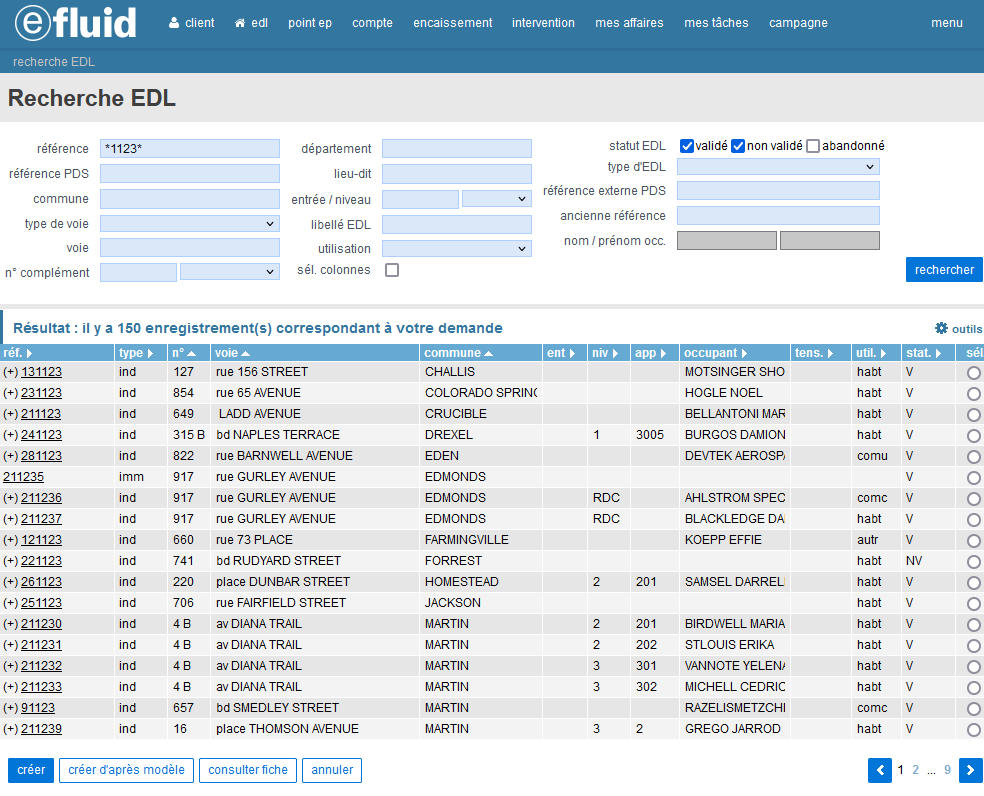
\includegraphics[height=9cm]{../res/efluid-2.png}
\end{center}

\chapter{\textit{Efluid} : organisation des services}
\label{appendix:efluid-organisation}

\begin{center}
  \begin{plantuml}
    @startmindmap
    
    <style>
      node {
          LineColor black
          BackgroundColor #FFF
          RoundCorner 0
      }
      arrow {
          LineColor #000
      }
      grey {
        BackgroundColor #BBB
      }
    </style>

      * Direction générale
      ** Direction informatique
      *** Technologies
      *** Développement : CRM et Facturation
      *** Développement : Comptage et réseaux <<grey>>
      ** Direction commerciale
      *** Expertise fonctionnelle : CRM et Facturation
      *** Expertise fonctionnelle : Comptage et réseaux
      *** Coordination et clients
      *** Prestation et projets
      ** Ginko

    @endmindmap
  \end{plantuml}
\end{center}

\vspace{1cm}
\noindent\textbf{CRM :} \textit{Customer Relationship Management}, gestion de la relation client.\\
\noindent\textbf{Ginko :} Service dédié à l'intégration d'\textit{Efluid} dans le SI d'\textit{Enedis}.

\chapter{\textit{Efluid} : gouvernance}
\label{appendix:efluid-gouvernance}

\begin{center}
  \begin{plantuml}
    @startmindmap
    
    <style>
      node {
          LineColor black
          BackgroundColor #FFF
          RoundCorner 0
      }
      arrow {
          LineColor #000
      }
      grey {
        BackgroundColor #BBB
      }
    </style>

      * Efluid
      **_ 60%
      *** UEM
      **_ 30%
      *** Enedis
      **_ 10%
      *** CDC

    @endmindmap
  \end{plantuml}
\end{center}

\vspace{1cm}
\noindent\textbf{UEM :} Usine d'Electricité de Metz.\\
\noindent\textbf{CDC :} Caisse des Dépôts et Consignations.

\chapter{Planification}
\label{appendix:planification}

\begin{itemize}
  \item \textbf{Planification générale du projet :}\\
\end{itemize}

\begin{center}
  \begin{plantuml}
    @startuml

    skinparam monochrome true
    scale 1024 width
    scale 768 height

    printscale monthly zoom 1.4
    project starts the 2020-09-01

    [Pré-conception] starts 2020-09-01
    [Pré-conception] ends 2020-12-31
    [Conception] starts 2020-12-01
    [Conception] ends 2021-05-31
    [Développements] starts 2021-03-01
    [Développements] ends 2021-08-31

    @enduml
  \end{plantuml}
\end{center}
\vspace{1cm}

\begin{itemize}
  \item \textbf{Planification détaillée :}\\
\end{itemize}

\begin{center}
  \begin{plantuml}
    @startuml

    skinparam monochrome true
    scale 1024 width
    scale 768 height

    printscale weekly
    project starts the 2021-02-01

    [Formalisation du besoin] starts 2021-02-01
    [Formalisation du besoin] ends 2021-02-15
    --
    [Intégration de la solution] starts 2021-02-08
    [Intégration de la solution] ends 2021-03-07
    --
    [Squelette batch] starts 2021-03-01
    [Squelette batch] ends 2021-03-15
    --
    [Implémentation des chargements] starts 2021-03-16
    [Implémentation des chargements] ends 2021-05-01
    --
    [Implémentation des process] starts 2021-04-16
    [Implémentation des process] ends 2021-06-01
    --
    [Tests] starts 2021-06-01
    [Tests] ends 2021-07-31

    [Squelette batch]->[Implémentation des chargements]
    [Implémentation des chargements]->[Tests]
    [Implémentation des process]->[Tests]
    [Intégration de la solution]->[Tests]

    @enduml
  \end{plantuml}
\end{center}

\chapter{Volumétrie}
\label{appendix:volumetrie}

\textit{Volumes estimés le 20/01/2021, sur une durée d'un mois, à partir des copies anonymisées des bases de données de production.}\\

Les données suivantes permettent d'évaluer le nombre de relèves concernées par le processus de demande de publication quel que soit leur contexte de création.\\

\begin{itemize}
  \item \textbf{UEM}
  \begin{itemize}
    \item \approx\space 3 500 relèves impliquant une création d'échange
    \item \approx\space 91 000 relèves créées
    \item Ratio demande de publication / création de relève : \approx\space 4\%
  \end{itemize}
  \item \textbf{Enedis IDF}
  \begin{itemize}
    \item \approx\space 6 300 000 relèves impliquant une création d'échange
    \item \approx\space 6 400 000 relèves créées
    \item Ratio demande de publication / création de relève : \approx\space 99\%
  \end{itemize}
  \item \textbf{Enedis Est}
  \begin{itemize}
    \item \approx\space 3 000 000 relèves impliquant une création d'échange
    \item \approx\space 3 100 000 relèves créées
    \item Ratio demande de publication / création de relève : \approx\space 95\%
  \end{itemize}
  \item \textbf{Enedis Ouest}
  \begin{itemize}
    \item \approx\space 5 200 000 relèves impliquant une création d'échange
    \item \approx\space 5 400 000 relèves créées
    \item Ratio demande de publication / création de relève : \approx\space 96\%
  \end{itemize}
  \item \textbf{Enedis Méditerranée}
  \begin{itemize}
    \item \approx\space 5 200 000 relèves impliquant une création d'échange
    \item \approx\space 5 400 000 relèves créées
    \item Ratio demande de publication / création de relève : \approx\space 96\%
  \end{itemize}
\end{itemize}
\clearpage

Les données suivantes permettent d'évaluer le nombre de relèves concernées par le processus de demande de publication en ne considérant que les relèves réalisées via un compteur \textit{\textit{Linky}}.\\

\begin{itemize}
  \item \textbf{Enedis IDF}
  \begin{itemize}
    \item \approx\space 5 400 000 relèves de compteurs \textit{\textit{Linky}} impliquant une création d'échange
    \item \approx\space 5 500 000 relèves de compteur \textit{\textit{Linky}} créées
    \item Ratio demande de publication / création de relève : \approx\space 98\%
    \item \approx\space 85\% des relèves créées concernent un compteur \textit{\textit{Linky}}
    \item \approx\space 85\% des demandes de publication de la relève concernent une relève de compteur \textit{\textit{Linky}}
  \end{itemize}
  \item \textbf{Enedis Est}
  \begin{itemize}
    \item \approx\space 2 500 000 relèves de compteurs \textit{Linky} impliquant une création d'échange
    \item \approx\space 2 600 000 relèves de compteur \textit{Linky} créées
    \item Ratio demande de publication / création de relève : \approx\space 95\%
    \item \approx\space 89\% des relèves créées concernent un compteur \textit{Linky}
    \item \approx\space 85\% des demandes de publication de la relève concernent une relève de compteur \textit{Linky}
  \end{itemize}
  \item \textbf{Enedis Ouest}
  \begin{itemize}
    \item \approx\space 4 600 000 relèves de compteurs \textit{Linky} impliquant une création d'échange
    \item \approx\space 4 800 000 relèves de compteur \textit{Linky} créées
    \item Ratio demande de publication / création de relève : \approx\space 96\%
    \item \approx\space 89\% des relèves créées concernent un compteur \textit{Linky}
    \item \approx\space 90\% des demandes de publication de la relève concernent une relève de compteur \textit{Linky}
  \end{itemize}
  \item \textbf{Enedis Méditerranée}
  \begin{itemize}
    \item \approx\space 4 800 000 relèves de compteurs \textit{Linky} impliquant une création d'échange
    \item \approx\space 4 900 000 relèves de compteur \textit{Linky} créées
    \item Ratio demande de publication / création de relève : \approx\space 97\%
    \item \approx\space 90\% des relèves créées concernent un compteur \textit{Linky}
    \item \approx\space 91\% des demandes de publication de la relève concernent une relève de compteur \textit{Linky}
  \end{itemize}
\end{itemize}

\chapter{Traitement de la demande de publication}
\label{appendix:process}

\begin{itemize}
  \item \textbf{Structure des traitements :}\\
\end{itemize}

\begin{center}
  \begin{plantuml}
    @startuml

    skinparam monochrome true
    left to right direction

    GestionDemandePublicationReleveProcess <|-- GestionDemandePublicationAvecDonneesProcess
    GestionDemandePublicationReleveProcess <|-- GestionDemandePublicationEstimationReleveFacturationProcess
    GestionDemandePublicationReleveProcess <|-- GestionDemandePublicationImportReleveAvecDonneesProcess

    @enduml
  \end{plantuml}
\end{center}
\vspace{0.5cm}

\begin{itemize}
  \item \textbf{Processus appelants :}\\
  \begin{itemize}
    \item Saisie d'une relève par un agent
    \item Auto-relève lors d'une demande de prestation
    \item CRI\footnote{Compte-Rendu d'Intervention} avec saisie d'une relève
    \item REL005MT : \textit{Batch} de calcul des consommations
    \item REL019MT : \textit{Batch} d'import des télérelèves gaz
    \item FAC002MT : \textit{Batch} d'estimation des relèves pour EDP\footnote{Elément De Population} facturable
    \item FAC006MT : \textit{Batch} de calcul des factures
    \item FAC020MT : \textit{Batch} d'estimation des relèves pour EDP non factuable
    \item \underline{LKY06} : Interface de récupération des données \textit{Linky}
  \end{itemize}
\end{itemize}

\chapter{\textit{Design Pattern}\footnote{Patron de conception} : Stratégie}
\label{appendix:strategy}

La stratégie est un patron de conception comportemental qui permet de définir des services et de les injecter de manière interchangeable dans un processus plus complexe. La mise en oeuvre de ce \textit{pattern} permet ainsi de respecter le principe OCP, \textit{Open/Closed Principle}\footnote{Principe ouvert/fermé}, qui garantit la bonne modularité du code. Ce principe suppose en effet qu'une entité (classe, fonction, module ...) doit être fermée à la modification directe mais ouverte à l'extension ; qu'il doit être possible, en d'autres termes, de complexifier certains traitements sans avoir à modifier fondamentalement les traitements existants.\\

\begin{itemize}
  \item \textbf{Sans stratégie :}\\
\end{itemize}

\begin{center}
  \begin{plantuml}
    @startuml

    skinparam monochrome true
    scale 200 height

    class Process {
      executer() : void
    }
    class SousProcess1 {
      executer1() : void
    }
    class SousProcess2 {
      executer2() : void
    }
    class SousProcess3 {
      executer3() : void
    }

    Process ..> SousProcess1
    Process ..> SousProcess2
    Process ..> SousProcess3

    @enduml
  \end{plantuml}
\end{center}
\clearpage

Ici, l'ajout d'un nouveau sous-process nécessite forcément l'adaptation du processus principal :\\

\begin{lstlisting}
public class Process {

    public void executer() {
        if (condition1) {
          new SousProcess1().exectuer1();
        } else if (condition2) {
          new SousProcess2().executer2();
        } else if (condition3) {
          new SousProcess3.executer3();
        }
    }    
}
\end{lstlisting}
\vspace{0.5cm}

\begin{itemize}
  \item \textbf{Avec stratégie :}\\
\end{itemize}

\begin{center}
  \begin{plantuml}
    @startuml

    skinparam monochrome true

    class Process {
      -service : Service
      +executer() : void
    }
    interface Service {
      +executerService() : void
    }
    class SousProcess1 {
      +executerService() : void
    }
    class SousProcess2 {
      +executerService() : void
    }
    class SousProcess3 {
      +executerService() : void
    }

    Process *-- Service
    Service <-- SousProcess1
    Service <-- SousProcess2
    Service <-- SousProcess3

    @enduml
  \end{plantuml}
\end{center}
\clearpage

Avec le respect du \textit{pattern}, un nouveau sous-process peut être injecté comme dépendance du processus principal, de la même manière que les processus existants. Aucune modification n'est donc nécessaire dans la classe principale :\\

\begin{lstlisting}
  public class Process {

      private Service service;

      public Process(Service service) {
        this.service = service;
      }
  
      public void executer() {
          service.executerService();
      }    
  }
\end{lstlisting}

\chapter{\textit{Batch} : architecture et implémentation}
\label{appendix:batch}

\begin{itemize}
  \item \textbf{Architecture :}\\
\end{itemize}

\begin{center}
  \begin{plantuml}
    @startuml

    scale 450 height
    skinparam monochrome true

    abstract class ProgramBatchDAO
    abstract class ProgramBatch
    class ParallelJobLauncher
    abstract class AbstractAppBatchJob
    abstract class BatchJobDAO

    ProgramBatch .u.> ProgramBatchDAO
    ProgramBatch .d.> ParallelJobLauncher
    ParallelJobLauncher .d.> AbstractAppBatchJob
    AbstractAppBatchJob .d.> BatchJobDAO

    @enduml
  \end{plantuml}
\end{center}
\clearpage

\begin{itemize}
  \item \textbf{Implémentation :}\\
\end{itemize}

\begin{center}
  \begin{plantuml}
    @startuml

    skinparam monochrome true
    scale 250 height

    class DemandePublicationRekeveProgramDAO #BBB
    class ERequeteDemandePublicationReleveBatchDAO
    class DemandePublicationReleveJobDAO #BBB

    DemandePublicationRekeveProgramDAO ..> ERequeteDemandePublicationReleveBatchDAO
    DemandePublicationReleveJobDAO ..> ERequeteDemandePublicationReleveBatchDAO

    @enduml
  \end{plantuml}

  \vspace{0.5cm}

  \begin{plantuml}
    @startuml

    skinparam monochrome true
    scale 150 height

    class DemandePublicationReleveProgram #BBB
    class DemandePublicationReleveBatchConstantes

    DemandePublicationReleveProgram ..> DemandePublicationReleveBatchConstantes

    @enduml
  \end{plantuml}

  \vspace{1cm}

  \begin{plantuml}
    @startuml

    skinparam monochrome true
    left to right direction

    class DemandePublicationReleveJob #BBB
    class GestionDemandePublicationReleveProcess
    class ECountDemandePublicationReleveType
    class DemandePublicationReleveBatchDAOExceptions

    DemandePublicationReleveJob ..> GestionDemandePublicationReleveProcess
    DemandePublicationReleveJob ..> ECountDemandePublicationReleveType
    DemandePublicationReleveJob ..> DemandePublicationReleveBatchDAOExceptions

    @enduml
  \end{plantuml}
\end{center}

\clearpage
\pagestyle{empty}
{
  \renewcommand{\thispagestyle}[1]{}
  \tableofcontents
}

\clearpage
\thispagestyle{empty}
\null
\vspace{1cm}
\begin{center}
  \LARGE\textbf{Mémoire de Licence Professionnelle}\\
  \vspace{0.3cm}
  \large\textit{Loïc STEINMETZ}\\
  \vspace{0.5cm}
  \rule{\textwidth}{0.4pt}
\end{center}
\vspace{0.5cm}

Ce mémoire présente les travaux menés dans le cadre de la Licence Professionnelle d'informatique mention Génie Logiciel. Cette formation a été réalisée en alternance à l'IUT de Metz et au sein d'\textit{Efluid}, société éditrice de logiciel également basée à Metz.\\

Le mémoire présente l'entreprise d'accueil, ses processus de production et l'environnement de développement mis en place dans les différents services. Il détaille en outre le projet industriel qui m'a été confié et qui consistait en l'implémentation de traitements de masse, gérés de manière asynchrone. Ces développements visaient notamment à réaliser des optimisations en matière de performance s'agissant du traitement de la relève des compteurs communiquants, ou compteurs \textit{Linky}.

\begin{figure}[b]
  \begin{center}
    
\includegraphics[height=2cm]{../res/logo-efluid.jpg}\\
    \rule{10cm}{0.2pt}\\
    \vspace{0.7cm}
    
\includegraphics[height=1.5cm]{../res/logo-iut.png}
  \end{center}
\end{figure}

\end{document}
